\documentclass[sigconf, timestamp-false, anonymous=true]{acmart}

\usepackage{listings}
\usepackage{multirow}
\usepackage{graphicx}
\usepackage{subcaption}
\usepackage{hyperref}
\usepackage{fancybox}
\usepackage{enumitem}

%% Rights management information.  This information is sent to you
%% when you complete the rights form.  These commands have SAMPLE
%% values in them; it is your responsibility as an author to replace
%% the commands and values with those provided to you when you
%% complete the rights form.
\setcopyright{none}

\acmConference[ESEC/FSE '20]{ESEC/FSE '20: ACM Joint European Software Engineering Conference and Symposium 
on the Foundations of Software Engineering}{November 8-13, 2020}{Sacramento, CA, USA}
\acmYear{2020}

\newcommand\todo[1]{\textcolor{red}{#1}}

%%
%% Submission ID.
%% Use this when submitting an article to a sponsored event. You'll
%% receive a unique submission ID from the organizers
%% of the event, and this ID should be used as the parameter to this command.
%%\acmSubmissionID{123-A56-BU3}

%%
%% The majority of ACM publications use numbered citations and
%% references.  The command \citestyle{authoryear} switches to the
%% "author year" style.

%%
%% end of the preamble, start of the body of the document source.
\title{A Study of Multi-Location Bug Patches}
\begin{document}



%add authors & shortauthors if we are lucky :)

\begin{abstract}
    Automatic program repair is a promising approach for reducing the
    cost of quality assurance practices and faulty software. To date, most
    techniques proposed for test-driven automatic repair have succeeded
    primarily on bugs that benefit from short, single-location patches. Techniques
    that successfully generate multi-location patches often do so in an
    alternative, single-edit way, or by targeting particular multi-location bug
    patterns. Empirical studies of real-world similarly tend to focus on the
    patterns exhibited by single-location bug patches, and have not examined repairability
    of multi-location patches in detail. We present a comprehensive empirical analysis
    of multi-location patches for bugs in open source Java programs, focusing on static and
    dynamic properties that define the repair search space for a given bug.
    This analysis focuses on the key challenges of the dynamic program repair
    problem: the \emph{mutations and fix code} used to repair bugs in multiple locations;
    the \emph{fault locations} and their relationships; and the \emph{objective
      function}, and in particular how and to what degree test cases can be used
    (or not) to identify partial repairs. We identify key takeaways and
    challenges, with implications for future work in expressive, multi-location bug
    repair.
\end{abstract}

%%
%% The code below is generated by the tool at http://dl.acm.org/ccs.cfm.
%% Please copy and paste the code instead of the example below.
\begin{CCSXML}
<ccs2012>
<concept>
<concept_id>10011007.10011074.10011099.10011102</concept_id>
<concept_desc>Software and its engineering~Software defect analysis</concept_desc>
<concept_significance>500</concept_significance>
</concept>
<concept>
<concept_id>10011007.10011074.10011784</concept_id>
<concept_desc>Software and its engineering~Search-based software engineering</concept_desc>
<concept_significance>500</concept_significance>
</concept>
</ccs2012>
\end{CCSXML}

\ccsdesc[500]{Software and its engineering~Software defect analysis}
\ccsdesc[500]{Software and its engineering~Search-based software engineering}

\keywords{software bugs, program repair}

\maketitle


\newcommand{\rqorinsight}[2]{
  \setlength{\fboxsep}{0.8em}
  \vspace{0.5em}
  \begin{center}
  \Ovalbox{\begin{minipage}{0.9\linewidth}
    \textbf{RQ#1:} #2
    \end{minipage}}
  \end{center}
  \vspace{0.5em}}

\section{Introduction}

Buggy software has a significant economic cost~\cite{cambridge-study}, and
software failures are estimated to have affected half of the world's
population~\cite{tricentis}. Software, and thus buggy software, has become
ubiquitous. The increased developer workload has motivated research in
techniques to automatically find and fix bugs, which have become integrated into
real-world development: Facebook now includes automated repair in their
production
environment.\footnote{https://engineering.fb.com/developer-tools/getafix-how-facebook-tools-learn-to-fix-bugs-automatically/}

A significant class of program repair techniques in both
research~\cite{genprog,angelix,Le17, Xuan17} and practice~\cite{sapfix} use test
cases to guide patch construction, typically by following what's known as a
generate-and-validate paradigm. At a high level, these techniques use test cases
to localize a defect --- identified by at least one failing test --- to a set of
likely-suspicious program locations. Then, they use a variety of techniques to
construct (or \emph{generate}) patch candidates for the bug in question,
checking each to see (or \emph{validate}) if any of them cause the program to
pass all of the provided test cases.
%
Patches are constructed in a variety of ways, ranging from heuristic, syntactic
program manipulation~\cite{par,genprog,rsrepair,ae,prophet,hdrepair}, to specially adapted program
synthesis techniques~\cite{Konighofer11,Konighofer12,semfix,DeMarco14,angelix}. These techniques have successfully
repaired real, meaningful defects in large, complex
programs~\cite{angelix,genprog-eight-dollars,prophet,sapfix}.

Practically speaking, these techniques are typically limited in the types and
variety of defects they can repair. Often this is by design: techniques may
limit the repair search space to single-location patches for
tractability~\cite{rsrepair,ae,hdrepair}, while others only target certain
classes of bugs~\cite{Xuan17,sapfix,DeMarco14,par}. However, even techniques
that can in principle generate repairs with multi-location patches typically
don't~\cite{genprog,others}.

This leaves a large proportion of real-world bugs unrepairable by modern
research techniques in program repair.  Over half of the bugs in popular bug
benchmark Defects4J are patched by humans using multi-part
patches~\cite{d4j-dissection}. Approximately 70\% of buggy source files in a
large study of bugs in Apache projects required edits at two or more
locations~\cite{zhong2015}.

A key tension in the design of an automated repair technique is the balance
between giving users confidence in patch correctness by maximizing its
subjective quality while managing a trivially-infinite search space. This space
is typically parameterized along several axes: (1) the \emph{fault space}:
potential program locations to be modified, (2) the \emph{mutation space}: which
modifications may be applied at a location, and (3) the \emph{fix space}: code
that may be instantiated for a specific mutation. For example, a repair
technique might identify the location of a null-pointer dereference (exploring
the fault space), decide to insert new code (mutation space), and synthesize
code to initialize the pointer (fix space). Many dynamic repair techniques can
be compared in terms of their choices along each of these axes, and traversal
strategies have first-order implications for scalability and for the type and
quality of patches produced. \todo{JL: I think a CT MBFL cite might be good here-ish.}

Multi-location repair poses distinct challenges for each of these axes for repair.
Spectrum-based fault localization~\cite{ochiai}, the most prevalent class of
fault localization techniques used in program repair, does not specifically
identify sets of locations that might be related or repaired together; indeed,
the evaluation of most fault localization techniques typicaly assumes that a bug
is localized if any one buggy line is identified~\cite{fl-survey-wong}.
Researchers have observed that some bugs are
repaired in multiple locations using very similar
code~\cite{saha2019harnessing,jiang2019cmsuggester}, informing novel techniques
that constrain the \emph{fix space} of possible multi-location repairs accordingly.
One key question for applicability of these types of techniques is how prevalent
such bugs are, and how often multi-location patches instead require multiple
coordinating (but ultimately different) edits or pieces of fix code.  Over 50\% of the fixes in four 
Apache projects involve two or more entities -- i.e., a Java class, method, or field -- and 66\%-76\% of 
those multi-entity fixes involved syntactic dependencies.~\cite{wang2018}. 
Test cases are used to evaluate candidate repairs in virtually all dynamic
generate-and-validate repair techniques, but, anecdotally, may not be effective
at identifying partial repairs in a multi-location
context~\cite{fitness10,maybeeric}.  
Although multi-location repair has been discussed in the context of other analyses
that study bug fix characteristics in general~\cite{examples} as well as for
repair applicability specifically~\cite{moar,examples}, to the best of our
knowledge there has been no significant previous study of the characteristics of
multi-location repairs in terms of their implications for repairability or, more
broadly, program repair.  

In this paper, we present a systematic study of real-world bugs with
multi-location patches,
looking specifically at their characteristics with respect to the problem of the
automatic repair search space.  
We study the bugs curated in two
real-world datasets that support program repair research: Defects4J~\cite{defects4j}
and BEARS~\cite{bears}, in total, 578 bugs in 40 projects. 
More than half of these bugs were repaired by a
human developer using edits at multiple locations.  We look at characteristics along each of the
relevant axes of the program repair search problem: fault locations, mutation
operators, fix code, and evaluation (or fitness or objective) using test cases.  Our 
contributions are
as follows:

\begin{itemize}
\item An analysis and enumeration of multi-location patches in Defects4J and Bears.
\item A study characterizing the coverage of failing tests on faulty locations
  as a means of testing whether the underlying hypothesis in current fault
  localization techniques still holds for bugs requiring multi-location
  patches. We find that 58\% of relevant bugs have faulty locations that are not
  covered by all failing tests, thus the underlying assumptions do not
  necessarily hold.
\item A study characterizing the relationship between fix code at different locations.  We 
find that half of bug patches contain dependent edits.
\item A study of code clones. We find that over 30\% of bugs with multi-location
patches have very similar edits applied to different locations, suggesting the viability of 
program repair techniques designed to utilize code clones. Moreover, bugs in which 
none of the faulty locations are covered by all failing tests tend to have code clones, 
suggesting a way to tell when we should use a program repair technique designed for code 
clones.
\item A study of test cases as a means of evaluating both partial and full
  multi-location repairs.  We find that one third of bugs with multi-location
  patches in Defects4j more than half in Bears do not require the edits at every
  location in their provided human patches to pass all test cases, suggesting that a 
  significant portion of patches have auxiliary or unneeded edits. We also found that test 
  case based validation methods can positively identify close to 40\% of partial repairs
  while less than
  15\% of partial repairs cause more test assertions to fail. Moreover, we found that the 
  granularity in which you measure the affect of a partial repair on a test suite (i.e., by 
  measuring assertions failed, methods failed, or classes failed) can have a significant 
  influence on the ability to identify a partial repair.
\item Differences between the Defects4J dataset and the Bears dataset. We identified a 
few cases where the results differ significantly between datasets. For example, in 
characterizing how failing tests cover faulty code, we discovered that Defects4J had 
significantly more likely to have bugs in which faulty locations were not covered by all 
failing tests than Bears. Similarly, Partial repairs were identified by failing tests more often 
in Defects4J than in Bears. These differences emphasize the value in evaluating program 
repair techniques against multiple different datasets.
\item A replication package, which we shall publish post-review.
\end{itemize}

\todo{The rest of this paper is organized as follows.  We provide background on
generate-and-validate program repair, with a focus on the key parameters of the
program repair search problem, in Section~\ref{sec:background}.  We describe the
results of our analysis in Section~\ref{sec:results}, with discussion of
implications as well as limitations in Section~\ref{sec:discussion}.  Related
work is discussed in Section~\ref{sec:related}; Section~\ref{conclusions}
concludes.}

\section{Key Concepts and Research Questions}
\label{sec:background}

\paragraph{Search spaces in automatic program repair.} Automatic program repair (APR) techniques aim to find patches for bugs in
programs.  We restrict attention to dynamic or test-case guided program repair,
which describes the majority of research advancements over the past ten years.
Such techniques take as input a program and a set of test cases that serve as
the oracle for program correctness.  At least one of those tests should be
failing, corresponding to the bug to be repaired.

At a high level, any APR technique aims to solve a search or optimization
problem, seeking a set of edits (or patch) to the program that will lead it to
pass all of the provided tests. The repair search space is typically defined
along the following axes:
\begin{itemize}

\item \emph{Fault space.} The first problem in fixing a bug concerns
  \emph{where} in the code modifications should be applied. Dynamic repair
  techniques begin by using test cases as input to a fault localization
  technique. Such techniques identify (and typically score) suspicious code
  based on which test cases execute which pieces of code. Although the
  particulars of the fault localization employed can vary, most APR use some
  variant of spectrum-based fault localization (SBFL)~\cite{ochiai} in this first
  step. The resulting computation defines the fault space, or the candidate
  locations or code entities considered for repair.

\item \emph{Mutation space.} The mutation space is the set of applicable
  modifications at a specific program location. Examples include GenProg's
  \emph{append}, \emph{replace}, and \emph{delete} mutation operators over
  statements~\cite{genprog-operators} and Nopol's condition replacement over
  \texttt{if} statements and missing precondition addition over non-branch and
  non-loop statements~\cite{Xuan17}.  A larger mutation space generates a richer
  search space with potentially more repairs, but increases its size
  combinatorially~\cite{long-search-spaces}.

\item \emph{Fix space.} Once a particular mutation is selected, code must be
  generated. The size fix space is often a function of the chosen mutation
  operator: for instance GenProg's \emph{delete} mutation can only delete an
  entire statement~\cite{genprog}, while PAR's \emph{Calling another method with
    the same parameters} mutation replaces a method call with any other method
  that takes the same number and type of parameters~\cite{par}.

\item \emph{Objective function.} After candidate patches are generated, we must
evaluate them in some way. The most common objective functions are test case based
(such as GenProg's fitness function \cite{genprog}), where passing more unit tests
is viewed as better. This approach, however, has problems, as individual correct edits do not
necessarily make the code pass more tests. This poses as a serious challenge for 
crafting correct multi-edit repairs. Attempts were made to tackle this problem
by incorporating program invariants into objective function alongside test results
\cite{dinglyu}, but no significant improvement in repair success rate was achieved. 

\end{itemize}



\paragraph{Multi-location bugs.} There are several plausible definitions of multi- vs. single-location bugs, with
implications for how they are studied. For the purpose of this study, we define
a \emph{patch location} as a contiguous sequence of edited lines of
code. Additionally, since we would like to observe the behavior of code as edits
are applied one-by-one, we combine two locations if one starts block with
\texttt{\{} and the other closes it with \texttt{\}} (as they are not
independent). We ignore changes to comments, whitespace, or import statements.

Alternative definitions may have bearing on our results.  We argue that this
definition is natural for the purposes of our study, which focuses in particular
on understanding larger bugs for the purposes of 
adapting, extending, or applying new program repair techniques to address them. 

\paragraph{Research questions.}  The parameterization of the program repair
search problems into multiple subspaces informs our empirical study of those
spaces for the purposes of understanding multi-edit repair.  We address the
following research questions:

\begin{enumerate}[label=RQ\arabic*:]
\item \emph{How prevalent are multi-location human patches are in Defects4J and Bears?}
\item \emph{Do failing tests cover different portions of the fault?}
\item \emph{How prevalent are dependencies between edited code?}
\item \emph{How often do code clones occur in bugs with multi-location
  patches? Is the existence of code clones in human patches correlated with specific
  patterns of fault localization?}
\item \emph{Do test cases fully capture the effects of multi-location patches?}
\item \emph{How well do test case based validation methods identify partial repairs?}

\end{enumerate}

\section{Dataset Characteristics}
\label{sec:data-rq1}

\begin{table*}
\begin{center}
\begin{tabular}{l | rrr  | rr | rr | rr}
\toprule
\multicolumn{10}{c}{\textbf{Defects4J}} \\
\midrule
Project & Bugs & Src (kloc) & Test (kloc) & \multicolumn{2}{c}{Multi-location} 
		& \multicolumn{2}{c}{Multi-test} & \multicolumn{2}{c}{Multi-location \&}\\
&&&&\multicolumn{2}{c}{bugs}&\multicolumn{2}{c}{bugs}&\multicolumn{2}{c}{Multi-test bugs}\\
\midrule
JFreeChart  & 26 & 193.3 & 74.6  & 11 & 42\% & 10 & 38\% & 7 & 27\%\\
Closure compiler & 133 & 150.6 & 112.6 & 55 & 41\% & 58 & 44\% & 31 & 23\%\\
Apache commons-lang & 65 & 57.8 & 47.4  & 32 & 49\% & 17 & 26\% & 13 & 20\%\\
Apache commons-math & 106 & 45.0 & 41.5 & 53 & 50\% & 28 & 26\% & 22 & 21\%\\
Mockito & 38 & 23.0 & 28.5 & 16 & 42\% & 18 & 47\% & 8 & 21\%\\
Joda-Time & 27 & 82.9 & 70.4 & 17 & 63\% & 13 & 48\% & 9 & 33\%\\
\midrule
All (Defects4J) & 395 & 552.6 & 375.0 & 184 & 47\% & 144 & 36\% & 90 & 23\%\\
\midrule
\multicolumn{10}{c}{\textbf{Bears (single-module)}} \\
\midrule
FasterXML-jackson-databind & 26 & 95.7 & 53.6 & 17 & 65\% & 4 & 15\% & 2 & 8\%\\
INRIA-Spoon & 62 & 66.2 & 30.8  & 39 & 63\% & 23 & 37\% & 18 & 29\%\\
spring-data-commons & 15 & 45.8 & 28.8  & 9 & 60\% & 6 & 40\% & 2 & 13\%\\
traccar-traccar & 42 & 47.9 & 8.6 & 24 & 57\% & 3 & 7\% & 2 & 5\%\\
30 other projects & 38 & - & - & 22 & 58\% & 36 & 95\% & 9 & 24\%\\
\midrule
All (Bears) & 183 & >255.6 & >121.8 & 111 & 61\% & 72 & 39\% & 33 & 18\% \\
\midrule
Combined (Defects4J \& Bears) & 578 & >808.2 & >496.8 & 295 & 51\% & 216 & 37\% & 123 & 21\%\\
\bottomrule
\end{tabular}
\end{center}
\caption{\label{tab:dataset-characteristics} Characteristics of the Defects4J (top) and Bears (bottom) datasets.}
\end{table*}

Our study requires a dataset of indicative, real-world,
multi-location defects.  We study both the defects in
Defects4J~\cite{defects4j} and Bears~\cite{bears}.  Table~\ref{tab:dataset-characteristics}
summarizes these datasets, both of which
consist of historical
bugs found in real world software projects. Defects4J contains 395 bugs from 
six Java software projects, and is a popular dataset for evaluating 
program repair tools that target Java~\cite{durieux-repair-them-all}.
The dataset's patches are manually minimized to isolate the bug fix 
and exclude non-repair edits such as refactorings and feature additions.

With any dataset, however, there is a risk associated that tools may overfit
to the defects in question, and there is evidence that this situation applies to
program repair and Defects4J~\cite{durieux-repair-them-all}. 
We thus also study bugs from Bears~\cite{bears}, 
a set of Java bugs derived from failed Travis-CI builds of GitHub projects. 
Bears offers 251 bugs from 72 software projects, providing a greater diversity of 
projects compared to Defects4J. 
Several projects in Bears, however, are structured as multi-module projects, 
which are not currently compatible with our automation tools.
We thus limit our analysis of Bears to 183 bugs from 30 single-module projects.


We start our analysis of multi-location patches by asking the following research question:
\rqorinsight{1}{How prevalent are multi-location human patches are in Defects4J and Bears?}

Table~\ref{tab:dataset-characteristics} lists the number and percentages of
multi-location patches in Defects4J and Bears. 
We find that multi-location patches comprise over half of Bears and almost half of Defects4J.
Although a multi-location human patch for a bug does not imply the 
non-existence of a simpler patch, the high proportion of bugs that have 
multi-location patches demonstrates the relevance of such bugs to fault localization and
program repair. 

Bears contains a greater proportion of 
multi-location patches compared to Defects4J. This may be the 
result of manual patch minimization in Defects4J~\cite{defects4j} 
and lack thereof in Bears.
Thus, some Bears patches may be multi-location as a result of additional 
changes added for non-repair reasons.


\section{Fault localization}

%% what are the claims, what are we studying, why are we studying it


Spectrum-based fault localization (SBFL) is the most commonly studied, as well as the most 
effective~\cite{zou2019empirical}, fault localization technique. It is a key
first step to characterizing the \emph{fault space} in automatic program repair,
narrowing the search space to a portion of the program more likely (based on
test case behavior) to correspond to the fault.  

\paragraph{SBFL Basics.} \todo{Serena, please add an explanation of how SBFL
  works; it's key to understanding the underlying assumption.  This should
  include references as appropriate.}

Given these basics, fundamentally, a core
assumption underlying SBFL is that \emph{failing tests execute buggy portions of 
the code relatively more often than passing tests.} Thus, if all failing tests execute a 
particular line of code, then that line of code is scored as more suspicious.
This assumption is well-suited to single edit repair. Indeed, the evaluation
of most SBFL techniques asks exactly the question of interest when considering a
technique's suitability for single-edit repair: how often does a given technique
correctly, highly rank individual buggy lines of code? 

Such evaluations, by and large, do not consider the implications of
suspeciousness scoring in a multi-edit repair context.  Instead, evaluations
typically consider a technique ``successful'' if it identifies \emph{any} of a
set of changed lines as highly-ranked or likely-suspicious.  While appropriate
for the question being asked in such evaluations, this does not address
suitability for multi-line program repair.  Identifying one of several buggy
locations is generally inadequate in a context where multiple locations must be
modified.  

Thus, in this research question, we investigate how well the SBFL assumption
applies to tests that identify multi-line bugs. We focus especially on
multi-line bugs that are associated with multiple tests; \todo{short explanation
  of the intuition why. This is a placeholder, I'm a bit tired and so this
  succinct explanation is escaping me.} If multiple tests all cover the multiple
modified locations well, then SBFL's core assumption holds and multi-edit repair
can expect to effectively make use of the off-the-shelf ranking these techniques
currently provide (indeed, this has been tried~\cite{angelix}). If not---that
is, if multiple tests exercise \emph{different} portions of the buggy
code---SBFL off-the-shelf will by definition be less effective in guiding APR to
correctly modifying multiple buggy locations at once.

Therefore, for multi-edit bugs with multiple identifying failing tests, do the 
different failing tests cover exactly the same patch locations, exactly 
disjoint path locations, or some combination?


\rqorinsight[2]{How well do multiple tests cover the multiple locations
  implicated in multi-edit bugs?}

\paragraph{Methodology}

Between both datasets, there are 60 total bugs that are both multi-edit and 
multi-test -- 45 in Defects4J and 15 in Bears. For each of these bugs, we used 
Jacoco to determine which of the chunks in the human patch were executed by each failing test. Using 
this coverage data, we categorized the bug as one of 
three coverage patterns: \textit{disjoint} for bugs in which no chunk is covered by all failing tests, 
\textit{same} for bugs in which all 
tests cover the exact same chunks of the patch, and \textit{overlap} for all 
other bugs, where some chunks are covered by all failing tests, but some chunks are only covered by a 
subset of failing tests.

\paragraph{Results}
The overall distribution is seen in Figure \ref{fig:coverage-all}. Over a third 
of the bugs were classified as disjoint, indicating that for a significant 
portion of bugs, the failing tests do not all execute any portion of the faulty 
code. In addition, another 22\% were classified as overlap. Thus, over half of 
the bugs that were both multi-edit and multi-test contained chunks that were 
not executed by all failing test cases.
2

\begin{figure}
	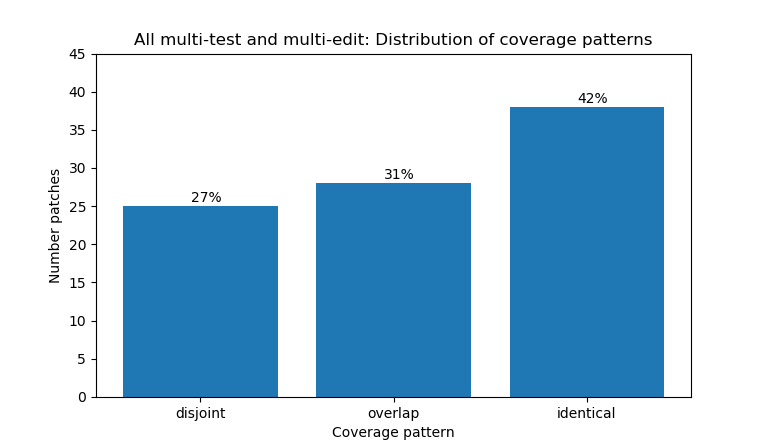
\includegraphics[width=\linewidth]{img/coverage-all.png}
	\caption{Distribution of coverage patterns for all multi-test and 
	multi-edit bugs in Bears and Defects4J. In all, 38\% of bugs were classified as disjoint, 40\% were 
	classified as same, and 22\% were classified as overlap.}
	\label{fig:coverage-all}
\end{figure}

SBFL assumes that faulty locations are executed more often by identifying 
or failing test cases and is not designed to find faults like these. Since SBFL 
is the most common fault localization technique in APR, most APR techniques 
are not well suited to fix a majority of these multi-edit and multi-test 
bugs.

If we divide distribution by dataset, we can see even more interesting 
behavior. Figure \ref{fig:coverage-datasets} shows the Defects4J dataset and 
the Bears dataset have very different distributions with respect to the 
disjoint and same categories -- in Defects4J, 47\% of bugs are disjoint and 
31\% are same, whereas in Bears, the proportions are 13\% disjoint and 67\% 
same. We hypothesize that this may be due to differences in how the two 
datasets were minimized, since Defects4J is a dataset of minimized and curated 
bugs while the bugs in Bears are taken scraped directly from the commits.


\begin{figure}
	\begin{subfigure}{\linewidth}
		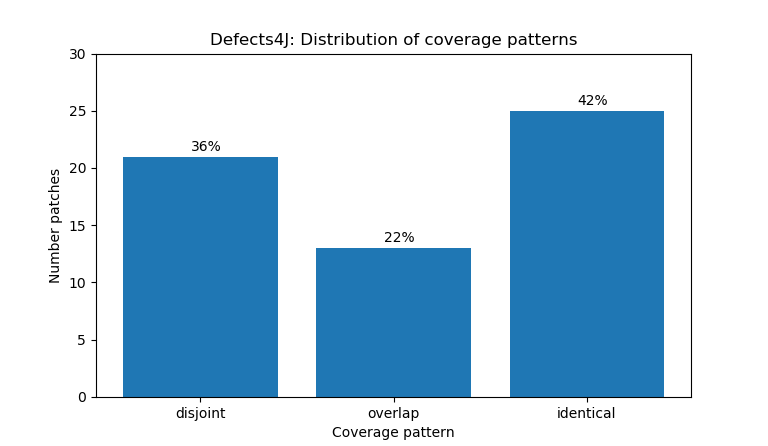
\includegraphics[width=\linewidth]{img/coverage-d4j.png}
		\caption{Distribution of coverage patterns for Defects4J. 47\% disjoint, 31\% same, and 22\% 
		overlap.}
	\end{subfigure}
	\begin{subfigure}{\linewidth}
		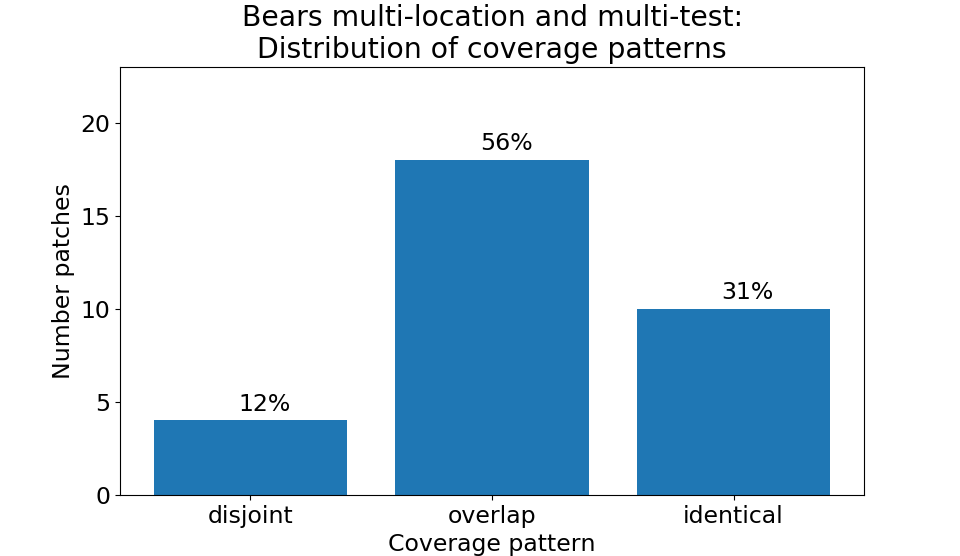
\includegraphics[width=\linewidth]{img/coverage-bears.png}
		\caption{Distribution of coverage patterns for Defects4J. 13\% disjoint, 67\% same, and 20\% 
		overlap.}
	\end{subfigure}
	\caption{Distribution of coverage patterns divided by dataset.}
	\label{fig:coverage-datasets}
\end{figure}


%\section{Symptoms}

We want to study symptoms in the context of fault localization. We define symptoms as the output given in failing test cases. In Java, most of these symptoms will be exceptions and their accompanying error message. Since most program repair is based off of failing tests, we want to see if those symptoms exhibited in those tests can correlate to type of repair.

For this paper, we specifically wanted to look at whether symptoms correlated with whether a bug could be fixed in a single location or multiple locations. If we can classify which bugs are single edit or multi edit, we can choose fault localization or patch generation techniques that are more suited.

We looked at all symptoms for all bugs in Defects4J and Bears, and categorized them based on whether they were one of the identified multi-chunk bugs or not. Then we fit the data to a linear regression model to see if there were statistically significant differences between the type of symptoms for multi edit and single edit bugs.

In order to find statistical significance, we needed to categorize the symptoms in big enough categories. We experimented with three groupings:

\begin{enumerate}
	\item Group all exceptions together except for assertion exceptions and exceptions for which a message indicates some sort of assertion (in our case, we simply looked for the keyword "expected"). We grouped the assertions into a few different types: 
	\begin{itemize}
		\item \lstinline{assert_null} is when the assertion is either expecting null, or got null when it wasn't expecting it.
		\item \lstinline{assert_int} is when the failing assertion was expecting a particular int value.
		\item \lstinline{assert_float} is the same as above, but for floats.
		\item \lstinline{assert_obj_arr_date} is when the assertion is expecting an object address, array of objects, or date object/date string. These are grouped together as commonly found but more complex assertions.
		\item \lstinline{error_expected} is when the failing test expected an exception, error, or warning.
		\item \lstinline{timeout} is when a Junit test times out, but also includes errors like stack overflows or out of memory exceptions.
		\item \lstinline{other_assert} for any other assertion that I couldn't easily categorize or parse. The large bulk of bugs in this category are bugs that had no error message at all; it simply failed with an \lstinline{AssertionError} or \lstinline{StackOverflow}.
		\item \lstinline{other}: all non-assertion exceptions.
	\end{itemize}
	\item Grouping symptoms together in an ad hoc way \todo{sell it better.}
	\begin{itemize}
		\item \lstinline{assert_prim}: assertions that compare to a Java primitive, such as int, float, or boolean.
		\item \lstinline{assert_null}: either expected or actual is null
		\item \lstinline{other_assert}: Asserting to anything that's not clearly a primitive or null.
		\item \lstinline{access}: all the bugs pertaining to wrongfully accessing or invoking certain fields or methods, or problems with classpath.
		\item \lstinline{null_pointer}: null pointer exceptions.
		\item \lstinline{timeout}: when a Junit test times out, but also includes errors like stack overflows or out of memory exceptions.
		\item \lstinline{parsing}: Anything related to parsing, serialization, or type conversion.
		\item \lstinline{other}: everything else
	\end{itemize}
	\item This last grouping is an even coarser version of the previous grouping.
	\begin{itemize}
		\item \lstinline{assert_equal}: Any assertion in which the test expected one value but got another
		\item \lstinline{other_assert}: any other assertion
		\item \lstinline{access}: all the bugs pertaining to wrongfully accessing or invoking certain fields or methods, or problems with classpath.
		\item \lstinline{null_pointer}: null pointer exceptions.
		\item \lstinline{parsing}: Anything related to parsing, serialization, or type conversion.
		\item \lstinline{other}: everything else
	\end{itemize}
\end{enumerate}

\todo{raw data from bogdan:}

assert only
\begin{lstlisting}
Call:
glm(formula = multi ~ assert_obj_arr_date + assert_int + assert_float + 
error_expected + timeout + assert_null + other_assert + other, 
family = "binomial", data = symptoms)Deviance Residuals: 
Min       1Q   Median       3Q      Max  
-1.2466  -0.5686  -0.4691  -0.4394   2.2880  Coefficients:
Estimate Std. Error z value Pr(>|z|)    
(Intercept)             -2.37550    0.38061  -6.241 4.34e-10 ***
assert_obj_arr_dateTRUE  1.24082    0.50907   2.437   0.0148 *  
assert_intTRUE           0.08619    0.45621   0.189   0.8502    
assert_floatTRUE         2.31273    0.48580   4.761 1.93e-06 ***
error_expectedTRUE       0.36735    0.53943   0.681   0.4959    
timeoutTRUE              0.99295    0.65378   1.519   0.1288    
assert_nullTRUE         -0.16611    0.58071  -0.286   0.7748    
other_assertTRUE         0.22402    0.36136   0.620   0.5353    
otherTRUE                0.63507    0.38201   1.662   0.0964 .  
---
Signif. codes:  0 '***' 0.001 '**' 0.01 '*' 0.05 '.' 0.1 ‘ ’ 1(Dispersion parameter for binomial family taken to be 1)    Null deviance: 546.49  on 645  degrees of freedom
Residual deviance: 510.11  on 637  degrees of freedom
AIC: 528.11Number of Fisher Scoring iterations: 5
\end{lstlisting}

grouping 1
\begin{lstlisting}
Call:
glm(formula = multi ~ access + assert_prim + null_pointer + timeout + 
assert_null + parsing + other_assert + other, family = "binomial", 
data = symptoms)Deviance Residuals: 
Min       1Q   Median       3Q      Max  
-0.9771  -0.6792  -0.5070  -0.4031   2.5944  Coefficients:
Estimate Std. Error z value Pr(>|z|)    
(Intercept)      -1.94778    0.36198  -5.381 7.41e-08 ***
accessTRUE        0.62756    0.41197   1.523   0.1277    
assert_primTRUE   0.81567    0.36223   2.252   0.0243 *  
null_pointerTRUE  0.32833    0.52496   0.625   0.5317    
timeoutTRUE       0.64782    0.63743   1.016   0.3095    
assert_nullTRUE  -0.52160    0.57971  -0.900   0.3682    
parsingTRUE       0.64081    0.50451   1.270   0.2040    
other_assertTRUE -0.03905    0.34777  -0.112   0.9106    
otherTRUE        -1.38263    0.76326  -1.811   0.0701 .  
---
Signif. codes:  0 '***' 0.001 '**' 0.01 '*' 0.05 '.' 0.1 ‘ ’ 1(Dispersion parameter for binomial family taken to be 1)    Null deviance: 546.49  on 645  degrees of freedom
Residual deviance: 523.84  on 637  degrees of freedom
AIC: 541.84Number of Fisher Scoring iterations: 5
\end{lstlisting}

grouping 2
\begin{lstlisting}
Call:
glm(formula = multi ~ assert_equal + access + null_pointer + 
parsing + other_assert + other, family = "binomial", data = symptoms)Deviance Residuals: 
Min       1Q   Median       3Q      Max  
-0.9390  -0.6809  -0.4377  -0.4377   2.2494  Coefficients:
Estimate Std. Error z value Pr(>|z|)    
(Intercept)       -2.0821     0.3470  -6.001 1.96e-09 ***
assert_equalTRUE   0.7532     0.3333   2.260   0.0238 *  
accessTRUE         0.7259     0.3979   1.824   0.0681 .  
null_pointerTRUE   0.4338     0.5131   0.845   0.3979    
parsingTRUE        0.7385     0.4976   1.484   0.1378    
other_assertTRUE  -0.2150     0.3223  -0.667   0.5048    
otherTRUE         -0.3646     0.5068  -0.719   0.4719    
---
Signif. codes:  0 '***' 0.001 '**' 0.01 '*' 0.05 '.' 0.1 ‘ ’ 1(Dispersion parameter for binomial family taken to be 1)    Null deviance: 546.49  on 645  degrees of freedom
Residual deviance: 527.48  on 639  degrees of freedom
AIC: 541.48Number of Fisher Scoring iterations: 5
\end{lstlisting}

In assert only, \lstinline{assert_float} correlates strongly with multiedit bugs. However, all the instances of \lstinline{assert_float} as a symptom occur in the Math package for Defects4J, and they all somehow to be multichunk. The sampling of \lstinline{assert_float} can be seenin the other two groupings as well, where \lstinline{asset_prim} and \lstinline{assert_equal}, both of which subsume \lstinline{assert_float}, are both more likey to be multi-edit.  \todo{take out math, redo analysis?}







\section{Mutation Operators and Fix Code}
\label{sec:mutops}

Given suitably selected fault locations, APR techniques vary in the types of
mutation operators they consider, how they select between them, and how they
select new fix code to instantiate them, as necessary.  For example, a na{\"i}ve
approach with only \texttt{insert}, \texttt{replace}, and \texttt{delete}
operators must choose between them at a location and, in the case of
\texttt{insert} and \texttt{replace}, choose code to insert/replace at that
location.  
%
The few techniques that handle or at least enable multi-edit patches vary in their
handling of mutation operator selection and instantiation.  At one
extreme, semantics-based repair~\cite{s3,angelix} can represent dependent edits between multiple
locations as a conjunction of multiple constraints to simultaneously solve,
bounded by some number of edits that are computationally feasible, while
restricted to a relatively small library of possible code components for use in
the inductive synthesis problem.    At the other extreme, search-based or
evolutionary techniques~\cite{genprog,others} typically treat different mutation
operators independently.  That is, a modification in one location does not
inform the selection of a modifications to apply in a second location; instead,
the heuristic search is trusted to identify copacetic combinations.  The size of
the search space increases combinatorially in this context, however, rendering
the chances of finding suitable multi-edit repairs without additional guidance
quite low~\cite{ae,long2016}. Accordingly, heuristic techniques targeted at multi-edit
repair contexts~\cite{hercules,maybewang2018} make assumptions about the
shape of the search space to render it tractably constrained --- in particular,
targeting bugs that can be repaired by multiple syntactically similar pieces of
fix code.

These kinds of targeted techniques surface the general questions about
multi-edit repairs we seek to answer, with
implications for how they should be designed in new techniques moving forward.
In particular, we want to examine the \emph{relationship} between multiple edits.

\subsection{Dependencies}

One of the dimensions of the relationship between multi-location patches is
\emph{dependency}. Specifically, we ask the following research question:
\rqorinsight{3}{How prevalent are dependencies between edited code?}

To answer this question, we broaden the scope of multi-location patches to 
include all patches containing at least two added, removed, or modified lines.
We consider a patch to contain dependent edits if there exists 
control or data dependencies between added, deleted, or modified statements.
We analyze deleted/modified statements in the pre-patch code 
and added/modified statements in the post-patch code for dependencies.
  
For practical performance and scalability reasons, 
we perform intraprocedural analysis. 
We do, however, gather some interprocedural data dependency information 
using the following heuristics:
\begin{itemize}
	\item If a statement invokes a method, then we assume that
	the statement reads all variables used in the method arguments.
	\item If a statement invokes a getter method \texttt{Class.getX()} 
	(for any \texttt{Class} and \texttt{X}), then we heuristically 
	assume that the statement reads \texttt{Class.X}. 
	Note that \texttt{Class.X} does not need to actually exist.
	\item If a statement invokes a setter method \texttt{Class.setX()}, 
	then we heuristically assume that the statement writes to \texttt{Class.X}. 
\end{itemize}

\paragraph{Results}

We find that 44\% of Defects4J patches, 61\% of Bears patches, 
and 49\% of the combined datasets' patches contain dependencies 
between edited statements.
Our finding supports earlier results on edit dependencies in 
bug patches~\cite{zhong2015}.
Patches with and without edit dependencies both form a substantial
portion of multi-line patches,
and neither type of patches should be ignored.

\begin{table}
{\begin{center}
	\begin{tabular}{l | rr | rr | rr}
		\toprule
		\multicolumn{7}{c}{\textbf{Patches with Dependent Edits}} \\
		\midrule
		APR & \multicolumn{2}{c}{Defects4J} & \multicolumn{2}{c}{Bears} & \multicolumn{2}{c}{Combined} \\
		\midrule
		Success & 39 & 30\% & 9 & 9\% & 48 & 26\% \\
		Failure & 93 & 70\% & 86 & 91\% & 139 & 74\% \\
		\midrule
		Total & 132 & 100\% & 95 & 100\% & 187 & 100\% \\
		\midrule
		\multicolumn{7}{c}{\textbf{Patches without Dependent Edits}} \\
		\midrule
		Success & 94 & 55\% & 8 & 13\% & 102 & 44\% \\
		Failure & 77 & 45\% & 53 & 87\% & 130 & 56\% \\
		\midrule
		Total & 171 & 100\% & 61 & 100\% & 232 & 100\% \\
		\bottomrule
	\end{tabular}
 \end{center}
}
	\caption{Number and percent of multi-line patches with respect to the presence of 
	dependent line edits and whether an APR tool successfully 
	repaired the bug in RepairThemAll~\cite{durieux-repair-them-all}.}
	\label{tab:dependency-repair-contingency-table}
\end{table}

To examine how the presence of edit dependencies may impact 
APR performance, we compare how often APR techniques 
successfully repair bugs whose patches do (not) contain edit dependencies.
Tables~\ref{tab:dependency-repair-contingency-table}
show the frequencies and percentages of multi-line patches with respect to edit dependency 
and whether an APR tool successfully repaired bug in 
RepairThemAll~\cite{durieux-repair-them-all}, a 
We find that the presence of edit dependencies 
reduces the likelihood of APR tool success for Defects4J bugs.
Using a $\chi^2$ test, we find a statistically significant relationship ($p < 0.001$)
between APR success and the presence of edit dependencies for Defects4J patches. 
We fail to find statistically 
significant relationships over only Bears patches, possibly due to the small number (16) of 
successfully auto-repaired Bears bugs with multi-line human patches.
The generally lower auto-repairability of bugs with edit dependent patches compared 
to their non-edit dependent brethren suggest that such dependencies indeed 
add complexity to the search for a repair.

\subsection{Cloned code}

In addition to dependency, multi-location patches can be related through syntactic
similarity. That is, a patch can consist of a code edit applied repeatedly in
multiple locations. Thus, we ask the following research question:

\rqorinsight{4}{How often do code clones occur in multi-location bugs? Is the existence of 
	code
	clones in human patches correlated with specific patterns of fault localization?}

Previous research ~\cite{wang2018} suggested that one potential way to enhance
APR techniques is to allow them to apply a single edits to multiple locations.
This is based on the observation that human developers tend to make exactly the 
same edits in multiple locations when fixing bugs. 

Therefore, as a proxy for measuring how often this style of repair occurs, we want to study the
prevalence of code clones in human patches. If a large proportion of multi-location bugs contains code 
clones, then we can corroborate the usefulness of previous repair techniques that specifically apply 
similar 
edits for a bug~\cite{saha2019harnessing}.

We will also attempt to correlate the coverage patterns outlines in Section \ref{secFL} with the 
existence of 
code clones in 
human patches. Intuitively, we might expect that a \emph{disjoint} bug may occur when a developer 
needs 
to apply the same fix at multiple independent locations; hence, we hypothesize that \emph{disjoint} 
bugs 
will have a higher incidence of code clones. In contrast, bugs categorized as \emph{same} or 
\emph{disjoint} may have more inter-related parts that are not merely the same statements copied to 
multiple locations.

In addition, if code clones occur more often with specific coverage patterns, the insights gained from 
fault 
localization can also help us identify the right repair technique --- i.e., if \emph{disjoint} bugs are more 
likely to have code clones, then we can use Wang et. al's suggestion to apply the same edits at multiple 
locations.

%Possible intuition: if we can find some kind of correlation between fault localization results
%and code clones, then if some APR research decided to follow Wang et al's suggestion and
%include "repeat same edits at multiple location" operator, then our results may advise
%the APR to be more likely to apply the repeat edit operator when the fault localization
%result matches specific patterns.

\subsubsection{Methodology}
\label{sec52}
We will look at the existence of code clones in multi-location bugs, including bugs in Closure (which are 
excluded from other experiments that require execution of tests), leaving 216 bugs to analyze. We 
excluded bugs with more than 6 faulty locations to constrain the search space.

In comparing these results with the results of the coverage experiment in
Section~\ref{secFL}, we will focus on the multi-test and multi-location bugs used in the coverage 
experiment, a total of 91 bugs.

We call the partial patches at two locations code clones if it is one of the following four cases
\begin{enumerate}
	\item Same Case: The two locations are alpha-equivalent. 
	\item Literal Case: The two locations differ by at most one constant or arithmetic operator,
	or replacement of one constant with variable 
	\item Composite Case: The patch at one location is exactly copied and contained within the patch at 
	the 
	second location (the second location  has additional lines in the patch).
	\item Move Case: Two locations forms a "movement" of code (i.e., one location is an insertion of 
	code 
	while the other is a deletion of the same code, essentially moving the code from one location to 
	another).
\end{enumerate}

\subsubsection{Results}

\begin{table}
{\begin{center}
\begin{tabular} {lrrr}
\toprule
& Defects4J & Bears & Combined \\
\midrule
Same & 35 & 9 & 44  \\ 
Literal & 11 & 2 & 13  \\
Composite & 7 & 1 & 8  \\
Move & 5 & 1 & 6  \\
\midrule
Any & 56 & 13 & 69  \\
No clones & 96  &  51 & 147 \\
Total & 152 & 64 & 216 \\
\% with Clones & 36.8\% & 20.3\% & 31.9\% \\
\bottomrule
\end{tabular}
\end{center}
}
\caption{Code clone information for multi-location bugs. 
     \emph{Same}, \emph{Literal}, \emph{Composite} and \emph{Move} corresponds to the
    four types of code clones considered, as described in Section~\ref{sec52}. ``Any'' means the bug
    contains any of the four types of clone; some bugs contain
    pairs of clones that belong to different categories. 
    Over
    30\% of multi-location bugs has code clones.}
\label{tab:clones}
\end{table}

As shown in Table~\ref{tab:clones}, out of the 216 multi-location bugs,
69 of them, or  32\%, included at least one type of cloning between fault locations, indicating a 
significant 
prevalence of code clones in multi-location human patches.
Note that "Any" may not
be the sum of the previous four rows because some bug could contain multiple pairs of code clones 
that
belong to different categories.


\begin{table}
{\begin{center}
\begin{tabular} {lrrrr}
\toprule
& Same Method & Same Class & Different Class & Total\\
\hline
Same & 24 & 18 & 5 & 47 \\ 
Literal & 9 & 4 & 1 & 14 \\
Composite & 3 & 5 & 0 & 8 \\
Move & 5 & 1 & 1 & 7 \\
\midrule
Total & 41 & 28 & 7  & 76\\
\bottomrule
\end{tabular}
\end{center}
}
\caption{
    Relative locations of sets of code clones in each category (defined in \ref{sec52}).
Same Method means the code clones occur in the same method, Same Class means the code
clones are in the same class but not in the same method, and Different Class means the
code clones are in different classes.
Shows that the majority of code clones occur within the same method
and majority of code clones are of ``Same'' category}
\label{tab:clones_loc}
\end{table}

As shown in Table \ref{tab:clones_loc}, over half of code clones are in the same method, while less than
one tenth of the code clones occur in different classes. Moreover, out of the 76 sets of code clones,
47 of them belongs to the ``same'' category, which means that 62\% of sets of code clones have completely
alpha-equivalent edit locations within them.

\begin{table}
	{\begin{center}
			\begin{tabular} {lrrrr}
				\toprule
				& Disjoint & Overlap & Identical & Total \\
				\midrule
				Has Clone & 19 & 2 & 5 & 26 \\
				No Clone & 6 & 26 & 33 &  65\\
                \midrule
				Total & 25 & 28 & 38 & 91 \\
                \bottomrule
			\end{tabular}
		\end{center}
	}
	\caption{Multi-location and multi-test bugs categorized on coverage patterns along the top 
	and code clones to the left. The coverage patterns are assigned based on how the failing 
	tests of a bug cover the different faulty locations. ``Disjoint'' refers to bugs in which none 
	of the faulty 
	locations were covered by all 
	failing tests.  ``Overlap'' refers to bugs with some faulty locations covered by all failing 
	tests, and 
	other faulty locations covered by a subset of failing tests. ``Same'' refers to bugs in 
	which the 
	failing tests all covered the exact same faulty locations.}
	\label{tab:cov_clones}
\end{table}

In Table \ref{tab:cov_clones}, we show the incidence of code clones among the three 
coverage patterns identified in Section \ref{secFL}. Note that out of 216 bugs evaluated for code clones, only 91 of them have multiple failing tests, so only these bugs are included in the table.  Out of 25 bugs labeled as 
\emph{disjoint} in the coverage 
experiment, 19 had code clones (14 Same, 4 Literal, 1 Composite). In contrast, the 
\emph{overlap} and \emph{identical} categories respectively had 2 and 5 bugs with code clones, 
making up only a small proportion of the bugs in those categories. This indicates that a 
bug with \emph{disjoint} coverage result is very likely to contain code clones in its
human patch. 

This result qualitatively supports the hypothesis that \emph{disjoint} bugs are more likely to contain 
code clones, while the other two classifications have comparatively less code clones. This suggests that 
future APR techniques to apply the same edits to multiple locations
if the coverage result of the bug can be categorized as \emph{disjoint}.


\section{Test case-based validation}

In search based program repair, one key area of research is to find ways to validate
candidate patches by
measuring how "close" a candidate patch is to a full repair (a fitness function),
and this is usually done via measuring unit test performance of the candidate patch. 

\rqorinsight{5}{Do test cases fully capture the effects of multiple edits?}

Sometimes not all edits in a human patch is necessary to pass all tests. This could be
due to human patch including refactoring or other changes that does not actually
change code behavior, or it could be due to the unit tests not being able to catch
an incorrect behavior that the remaining edits correct. We would like to explore
to what extent does this phenomenon affect the bugs in our benchmarks.

\rqorinsight{6}{How well do test case based validation methods identify partial repairs?}

Given a buggy program and a valid repair, if we apply a part of the valid repair to 
the buggy program (a partial repair), then semanticly the partial repair is closer
 to the full repair compared to the original. 
Ideally, we would want the fitness function to guide the search towards a full 
repair by identifying partial repairs as "closer" to full repair than original.

However, sometimes partial repairs will perform no different in unit tests compared 
to the original program, and other times they could perform worse. We want to find 
out how often each of these situations happen.

Moreover, unit test performance can be measured in different granularity levels. 
We would like to compare the performance of the fitness functions at identifying 
partial repairs at different granularity levels.


\subsection{Methodology}
\label{sec:partial-repair-methodology}

To address RQ5 and RQ6, we designed the following experiment: for each bug in 
Defects4j 
(excluding Clojure bugs because they dont use JUnit) 
and Bears (single-module only), we generate all of its partial repairs using method described in 
the Partial Repairs subsubsection, and then run unit tests through all partial repairs
as well as the original buggy program on three different granularity levels (described
in details in the Granularity subsubsection), and compare the results.

\subsubsection{Partial Repairs}

To construct partial repairs for each bug, we apply a struct, non-empty subset 
of location-granularity edits from the human patch to the broken code.
In order to minimize the number of syntactically invalid partial repairs, 
we pre-add, prevent the deletion of, or prevent the narrowing of scope of 
import statements, helper methods, and variable declarations.
For example, if a patch contains an edit location that declares a new variable 
\texttt{var} and a second edit location that might use \texttt{var}, then we 
pre-add the declaration of \texttt{var} from the first edit location. 
We argue that the semantic behavior of partial edits is more interesting 
than their syntactic correctness, which prompts us to apply the 
aforementioned preprocessing.

We do not split edit locations into two when applying any of our preprocessing steps. 
If an edit location, however, only contains edits that we pre-apply or remove during 
preprocessing, then we discard the now-empty edit location from the set of 
potential edits to apply. We eliminate bugs whose human patches contain only 
one edit location after preprocessing (for example, a 2-location patch that adds a new 
helper method in one edit location and invokes the helper method in the other). 

Due to the exponential growth of the number of partial repairs with respect 
to the number of available edit operations, we evaluate bugs whose patches 
contain between two and six edit locations after preprocessing.
Moreover, we exclude Defect4J's Closure compiler bugs due to 
their nonstandard test suite setup.
We are left with 97 Defects4J and 64 Bears bugs, a total of 898 partial repairs for Defects4j 
and 444 partial repairs for Bears.

\subsubsection{Granularity}

There are different ways to compare unit test results, and the most common ways 
are class-level granularity and method-level granularity. At Class-level granularity, 
we only look at which test classes passed and which failed; at method-level 
granularity, we look at which test methods passed and which failed.

Here we introduce a third level of granularity: assertion-level granularity. 
For each test method $M$, let $A(M)$ be the set of all assert statements in $M$. 
When $M$ is run, if an assertion failed, the failure is recorded and the method 
is allowed to continue to run (as opposed to normally the test method throws an 
error and terminates). After running the method, for each assert statement 
$a\in A(M)$, let $b(a)$ be 1 if $a$ never failed once during the running of $M$, 
and 0 otherwise. We define the assertion score of $M$ to be 
$AS(M)=\frac{\Sigma_{a\in A(M)}b(a)}{|A(M)|}$. If $M$ failed to run to completion 
due to timeouts or exceptions that are not related to assertions, then we define 
$AS(M)=0$. Thus by definition, $AS(M)=1$ if $M$ passes. If a program passed more 
assertions in $M$, there should be an increase in $AS(M)$.


\subsection{Results}

To answer RQ5, we report that about a 
third (32 out of 97) of Defects4j bugs and over half (34 out of 64) of
Bears bugs in this experiment do not need all edit locations in the provided human patches 
to pass
all unit tests. This suggests that significant portion of multi-location bugs contains some
edit locations that has completely no effect on the test case behavior. This could be due to a 
human developer refactoring code that doesn't change code behavior, which is a 
phenomenon that has been studied in previous work~\cite{tangledchanges}. This would 
suggest that bug benchmarks that rely on real bugs differ from the expected behavior and 
functionality of program repair techniques. Another reason for the seemingly extraneous 
partial repairs could be due to test cases not being able to detect incorrect behavior that is 
fixed
by the "unnecessary" edit location, which could elicit particular drawback to using tests as an 
oracle.

Due to the phenomenon above, we decided to present the results for RQ6 in two ways: 
always view full provided human patch as full repair
(Unminimized), and viewing minimum set of edit locations in provided human patch necessary
to pass all unit tests as full repair (Minimized).
Some bugs ends up with one edit location after minimization, 
so they are not included in the Minimized results. The minimized results 
include 75 remaining bugs (544 partial repairs) in defects4j and 38 remaining bugs (156 partial repairs) of Bears. 

Since each bug may have different 
number of partial repairs, we analyzed the results with the partial repairs weighted such that each bug
has equal weight, so if a bug has n partial repairs each of them has weight 
$\frac{1}{n}$. We record the percentage of partial repairs that performed better (positive), same (neutral)
or worse (worse) compared to original code in each assertion level. Non compiling
partial repairs do not count towards any of the three categories.

The full unminimized and minimized results in Table \ref{yiweitable}.


\begin{table}
{\begin{center}
\begin{tabular}{ll|rr|rrrr}
\toprule
\multicolumn{2}{c}{}&\multicolumn{2}{c}{Defects4j} & \multicolumn{2}{c}{Bears} \\
\multicolumn{2}{c}{Minimized?} & \multicolumn{1}{c}{No} & \multicolumn{1}{c}{Yes} & \multicolumn{1}{c}{No} & \multicolumn{1}{c}{Yes}  \\
\midrule
\multirow{3}{*}{Positive} & Class & 20.46\% & 9.78 \% & 27.60\% & 10.59\%  \\
 & Method & 41.25\% & 36.80 \% & 31.29 \% & 19.71\%  \\
 & Assertion & 48.25\% & 45.91 \% & 31.60 \% & 20.24\%  \\ 
\midrule
\multirow{3}{*}{Neutral} & Class & 65.53\% & 73.56 \% & 56.84 \% & 73.75\% \\
 & Method & 39.33\% & 39.95 \% & 51.60 \% & 64.62\%  \\
 & Assertion & 31.73\% & 30.30 \% & 47.48 \% &  59.19\%  \\ 
\midrule
\multirow{3}{*}{Negative} & Class & 7.18\% & 7.64 \% & 6.70 \% & 10.84\%  \\
 & Method & 12.52\% & 14.13 \% & 8.26 \% & 10.84\%  \\
 & Assertion & 12.90\% & 14.39 \% & 11.29 \% &  14.44\%  \\ 
\bottomrule
\end{tabular}
\end{center}}
\caption{Results of partial repairs using test case results
at all granularity levels.
More granular fitness functions are generally better at positively identifying partial repairs.}
\label{yiweitable}
\end{table}


Under highest granularity, we are able to identify above 45\% of the partial repairs in Defects4j
and above 20\% of the partial repairs in Bears. Only about 30\% of Defects4j partial repairs and 50-60\%
of Bears partial repairs are neutral and below 15\% of bugs in both datasets are negatively identified. This shows that, 
under high granularity, test case results can be a reasonably good indicator of partial repairs, as it makes much
more positive partial repair identifications than negative ones.
 
The experiment result shows that higher granularity levels are better at identifying partial repairs positively, 
but they also increase the chance of identifying partial repairs negatively.
This tradeoff can behave differently on different datasets. For example,
Assertion Level Granularity performed much better than Method Level Granularity
in Defects4j (close to 10\% more positively identified partial repairs, with less than
0.5\% more negatively identified), but this is not the case in Bears (less than 0.6\%
more positively identified partial repairs, with about 4\% more negatively identified).
Thus, it is recommended that researchers should 
carefully balance the tradeoffs in granularity level in test case based validation
in APR research.


\section{Limitations and Threats}

\todo{Please list all limitations and threats you can think of for your experiments, in 
something approaching a reasonable order, so we can integrate.  If you can, pull that 
discussion from previous sections, I didn't look for it beyond test cases.}

\paragraph{Coverage}

There are statements that Jacoco can't get coverage for, like inserted cases for switch 
statements, inserted else statements, method signatures, and other things that are compiled 
away in bytecode. We might have been able to get around these with some engineering 
effort, but since our focus is on how the coverage of different failing tests compared to each 
other, we felt that using Jacoco's coverage was a good enough approximation.

\paragraph{Dependency analysis.}
Since we use intraprocedural control and data dependency analysis, 
we may miss certain interprocedural dependencies between edited statements.
Although our heuristics for method invocations may account for certain 
interprocedural data dependencies, these heuristics may also introduce 
false positive data reads and writes, which may lead to inaccurate determinations 
of dependency.

\paragraph{Code clones.}

This experiment only looks at location level code clones, 
but there could also be code clones within a single edit 
location. This experiment also defined code clones with four categories 
(Same, Literal, Composite, Move), and there could be other categories as well. 

A set of code clones could contain two or more locations with similar edits, 
but we did not 
distinguish the actual number of edit locations in the experiment and treated all of them
as just one set of code clones.

\paragraph{Partial repair construction.}
The construction of partial repairs, as described in 
Section~\ref{sec:partial-repair-methodology},
 breaks up full repairs into locations and treats each edit location as a 
single edit action. However, in reality most APR techniques mutate code at 
a more granular level.
Also, this experiment only checks whether fitness functions 
can identify partial repairs, and not concerned with how to come up with these 
partial repairs (depending on specifics of the APR 
techniques, some may not be in the search space).

Regardless of its limitations, this experiment is provides valid and valuable 
information to tackling the challenge of automatically repairing bugs that 
requires multiple edit actions to fully repair 
and provides insight in future APR research.




\section{Related Work}

\cite{zou2019empirical}: Empirical study on fault localization, SBFL is the most effective standalone 
technique, except for faults with crashes, in which stack trace analysis is the most effective. They 
also combined different fault localization techniques by training a machine learning model, 
specifically using a learning to rank model. Their learning to rank model outperformed all the 
individual fault localization techniques. In their analysis, they considered a multi-edit bug to be 
localized if any faulty line is localized.

\cite{pearson2017evaluating}: Empirical study of multiple SBFL and mutation based faultlocalization 
techniques on Defects4J. Since many of these techniques were evaluated with artificial faults, the 
authors look at whether their effectiveness on artificial faults translates to effectiveness on real 
faults. This is not the case. They also show that SBFL outperforms mutation based fault localization.

Qi et al.~\cite{patch-correctness} evaluated the patches generated 
by three G\&V repair tools~\cite{genprog, ae, rsrepair} and presented 
Kali, a G\&V tool that exclusively deletes functionality. They found the 
vast majority of generated patches to be incorrect and equivalent to 
a single functionality deletion. Moreover, they found that Kali, whose 
smaller search space consists entirely of functionality-removing 
operations, generates at least as many correct patches as the 
other three tools. Later work found patch incorrectness to be 
also problematic in Defects4J~\cite{d4j-eval} and in semantics-based 
repair techniques~\cite{Le2018}.

% I know I'm referring to the work by the authors' names,
% but I can't find a good way to refactor their names out without writing awkwardly.
% I would need to refactor all of the usages of "they" to remove their names.
Long and Rinard~\cite{long-search-spaces} studied the prevalence of 
correct and incorrect plausible patches in the search spaces of SPR~\cite{spr} 
and Prophet~\cite{prophet}. They found incorrect plausible patches to outnumber 
correct patches by orders of magnitude. When they increased the search space 
by adding additional mutation operations, they found an increased number of 
correct patches, but APR tool performance might actually degrade due to a 
simultaneous increase in incorrect plausible patches and the combinatorial 
growth of the search space.

Zhong and Su~\cite{zhong2015} did an empirical study on real bug fixes. 
They studied the difficulty of fault localization, the complexity of fixing bugs, 
necessary mutation operators, importance of API knowledge, the types of buggy files, 
and addition/deletion of files in bug fixing on over 9000 real-world bugs collected via BUGSTAT, 
and identifies key insights on fault localization, faulty code fix, search space and non-source bugs. 
Both our paper and Zhong and Su's paper aims to provide useful guidance and insights for 
improving state-of-the-art APR techniques through empirical studies of bugs and bug fixes. 
In contrast, our study focuses on one specific category of bugs: 
source file bugs that requires multiple edit actions to successfully repair, 
drawing insights on their behaviors in fault localization, fitness evaluations and dependency.

Wang et al.~\cite{wang2018} did an empirical study of multi-entity changes in real bug fixes 
(where each entity is a class, method or field). Their research questions mostly focused on 
how often and why do real-world bug fixes have multi-entity changes, the relationship 
between co-changed entities, and the recurring patterns of those multi-entity changes. 
Through analyzing 2854 real-world bugs from four projects, they found that 66\%-76\% 
multi-entity fixes are closely related to each other via syntactic dependencies, 
and they identified three major recurring patterns that connects co-changed entities. 
They suggested a potential way to close the gap between APR fixes and real fixes by 
enhancing APR to incorporate multi-entity changes. In contrast, our study on bugs that
requires multiple edits to fix, where the edits may be in the same entity. We define atomic 
changes (single edit) differently, and we studied interactions between edits 
(i.e. the lines that changed in the bug fix) instead of entire entities.

Previous efforts in G\&V program repair to derive more search-guiding information 
during candidate patch evaluation 
include using program invariants~\cite{better-fitness, dinglyu}, 
intermediate program values~\cite{source-code-checkpoint}, 
and online mutation-based fault localization~\cite{mut-analysis}.
Some approaches require additional input, such as suspicious variables~\cite{source-code-checkpoint} 
or known patches for the bug under repair~\cite{better-fitness}, 
while others exhibit limited performance improvements~\cite{dinglyu, mut-analysis}.
Our work shows the potential benefit of using more granular objective functions such as
assertion level granularity compared to class/method level granularity, and maybe
future research can look into even more granular objective functions such as sub-assertion
level (different assert distance in AssertEqual, etc).

Schulte et al.~\cite{schulte} did an empirical study on software mutation robustness 
(i.e. how often do code mutations remain neutral in test results). 
They found that in a large collection of off-the-shelf softwares the mutation robustness is about 37\%, 
and discussed potential application of mutation robustness to proactive bug repair. 
In contrast, our study focuses on automatically fixing current bugs (i.e. bugs that fail an existing unit test), 
and we do not restrict our repair actions to neutral variants of the program.

\section{Conclusions}
\label{sec:conclusions}

\todo{Write me, plz, summarize takeaways and why we care.  We have established a
  roadmap of research directions for multi-edit repair.}

In conclusion, \todo{Fill sec 3 conclusion}

In assessing the validity of assumptions underlying SBFL in reference to multi-location 
bugs, we found that 58\% of bugs that were multi-location and had multiple failing tests 
had faulty locations 
that were covered by some but not all the tests. In addition, 27\% of multi-location and 
multi-test patches  This indicates that the assumption underlying SBFL, namely that faulty 
locations in the code are executed more often by failing tests, does not necessarily hold 
for multi-location patches. Thus, we need to develop alternative fault localization 
techniques that are scalable and effective for multi-location patches.

We characterized the relationships between multiple edits in a bug
We find that approximately half of multi-edit bugs 
contain dependent edits in their human patches, and such bugs may be more 
difficult for APR techniques to repair.
We also find that over 30\%
of multi-location bugs have some kind of code clones, making code clones fairly prevalent 
among bugs. Moreover, we found that multi-location bugs that were found to be 
\emph{disjoint} in our coverage analysis (i.e., had no location that was executed by all 
failing tests) were more likely to be code clones. This indicates that program repair 
techniques that focus on fix patterns based on code clones are viable for a significant 
portion of bugs. In addition, since code clones are more common in bugs with certain 
patterns of coverage, we can use that in fault localization and patch generation to identify 
which bugs would benefit most from the aforementioned program repair techniques.

In measuring how test cases respond to the application of partial repairs, we found that 
test case based validation methods can be reasonably good at identifying partial
repairs at when measuring the effect of the partial repair on the test suite at a higher 
granularity level such as method level or assertion level. This suggests that for a generate 
and validate program repair approach, applying a partial patch can still guide the approach 
towards the correct patch. Moreover, 
we observed that the number of both positively and negatively identified partial repairs
increase as we increase the granularity, so we advise a careful balance of the tradeoffs of
granularity levels in future search based APR development.

As an additional insight gained from measuring test case response to partial patches, we 
also found that test case based validation methods cannot capture all effects of human 
patches,
as between a third and a half of multi-location bugs are still able to pass all the tests 
without all partial patches being present. This builds on previous work and motivates 
future work on the minimality of human patches.

These findings have implications for using program repair for multi-location bugs, both in 
terms of how existing program repair techniques can repair multi-location bugs and how 
we should design future repair techniques.

To ensure reproducibility and encourage further investigation, we intend to release a 
replication package post-review.

\bibliographystyle{ACM-Reference-Format}
\bibliography{references}

\end{document}
\endinput
